% !TEX TS-program = pdflatex
\documentclass[12pt]{article}
\usepackage[margin=1.5cm]{geometry}
\usepackage{tikz}
\usetikzlibrary{shapes.geometric,positioning,shadows,fit}

\pagestyle{empty}
\newcommand{\Lam}[1]{\section*{#1}\vspace{-1ex}}

\tikzset{
	titulo/.style={rectangle, rounded corners, fill=purple!70!black, 
		text=white, font=\bfseries\LARGE, minimum width=12cm, 
		minimum height=1.5cm, text centered, drop shadow},
	nivel1/.style={rectangle, rounded corners, fill=teal!80!black, 
		text=white, font=\bfseries\Large, minimum width=9cm, 
		minimum height=1cm, text centered, drop shadow},
	nivel2/.style={rectangle, rounded corners, fill=black!60, 
		text=white, font=\large, text width=8.5cm, 
		minimum height=0.8cm, align=left, drop shadow}
}

\begin{document}
	
	% =========================================================
	\Lam{Lámina 1 — Flechas y conectores}
	\begin{center}
		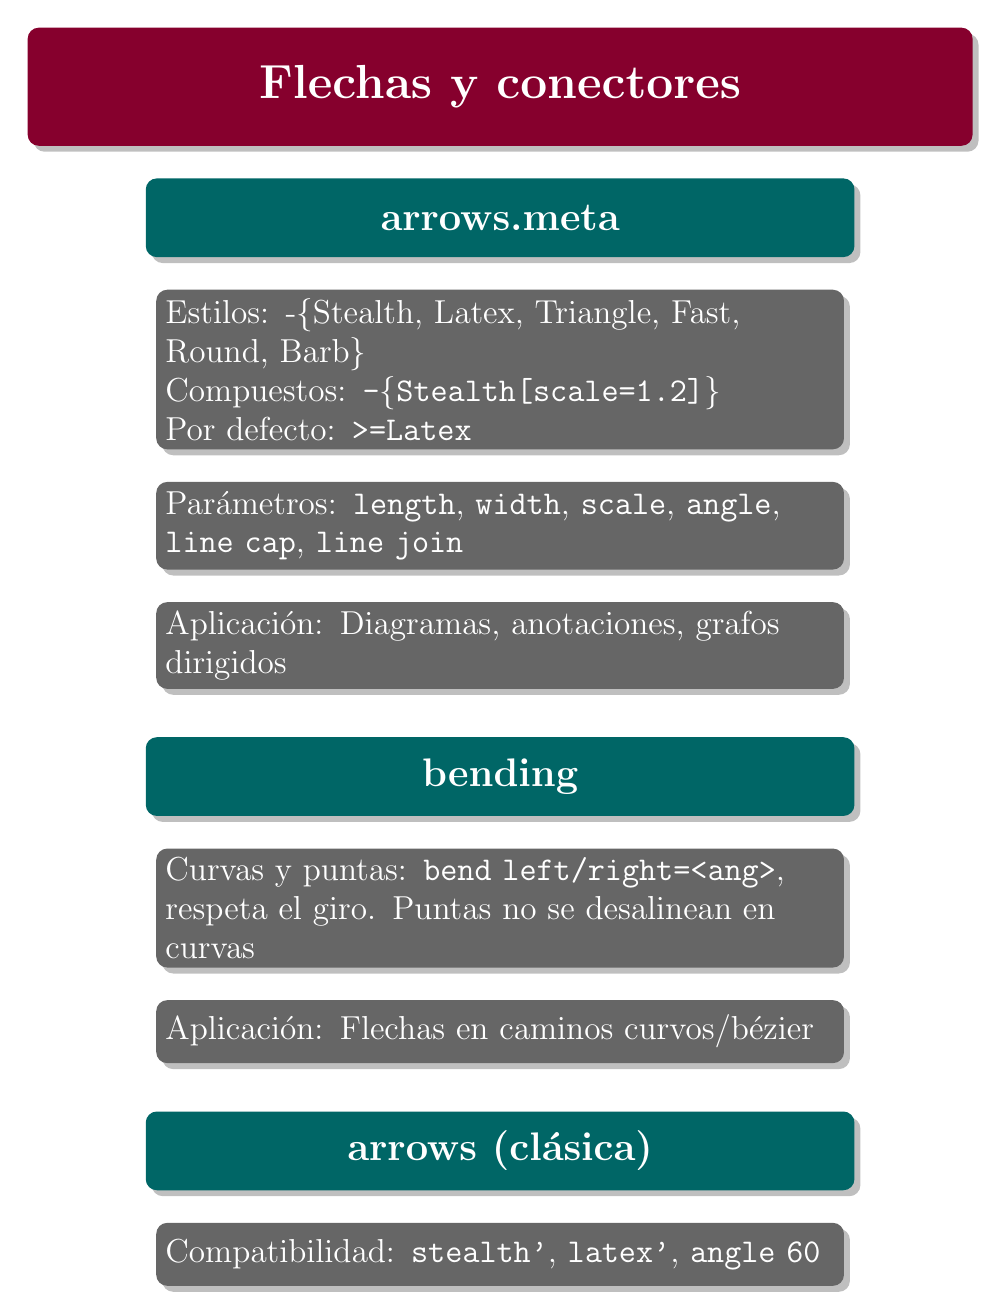
\begin{tikzpicture}[node distance=0.4cm]
			\node[titulo] (root) {Flechas y conectores};
			
			\node[nivel1, below=of root] (arrows) {arrows.meta};
			\node[nivel2, below=of arrows] (a1) {Estilos: -\{Stealth, Latex, Triangle, Fast, Round, Barb\}\\
				Compuestos: \texttt{-\{Stealth[scale=1.2]\}}\\
				Por defecto: \texttt{>=Latex}};
			\node[nivel2, below=of a1] (a2) {Parámetros: \texttt{length}, \texttt{width}, \texttt{scale}, \texttt{angle}, \texttt{line cap}, \texttt{line join}};
			\node[nivel2, below=of a2] (a3) {Aplicación: Diagramas, anotaciones, grafos dirigidos};
			
			\node[nivel1, below=0.6cm of a3] (bending) {bending};
			\node[nivel2, below=of bending] (b1) {Curvas y puntas: \texttt{bend left/right=<ang>}, respeta el giro. Puntas no se desalinean en curvas};
			\node[nivel2, below=of b1] (b2) {Aplicación: Flechas en caminos curvos/bézier};
			
			\node[nivel1, below=0.6cm of b2] (classic) {arrows (clásica)};
			\node[nivel2, below=of classic] (c1) {Compatibilidad: \texttt{stealth'}, \texttt{latex'}, \texttt{angle 60}};
		\end{tikzpicture}
	\end{center}
	
	% =========================================================
	\Lam{Lámina 2 — Posicionamiento y coordenadas}
	\begin{center}
		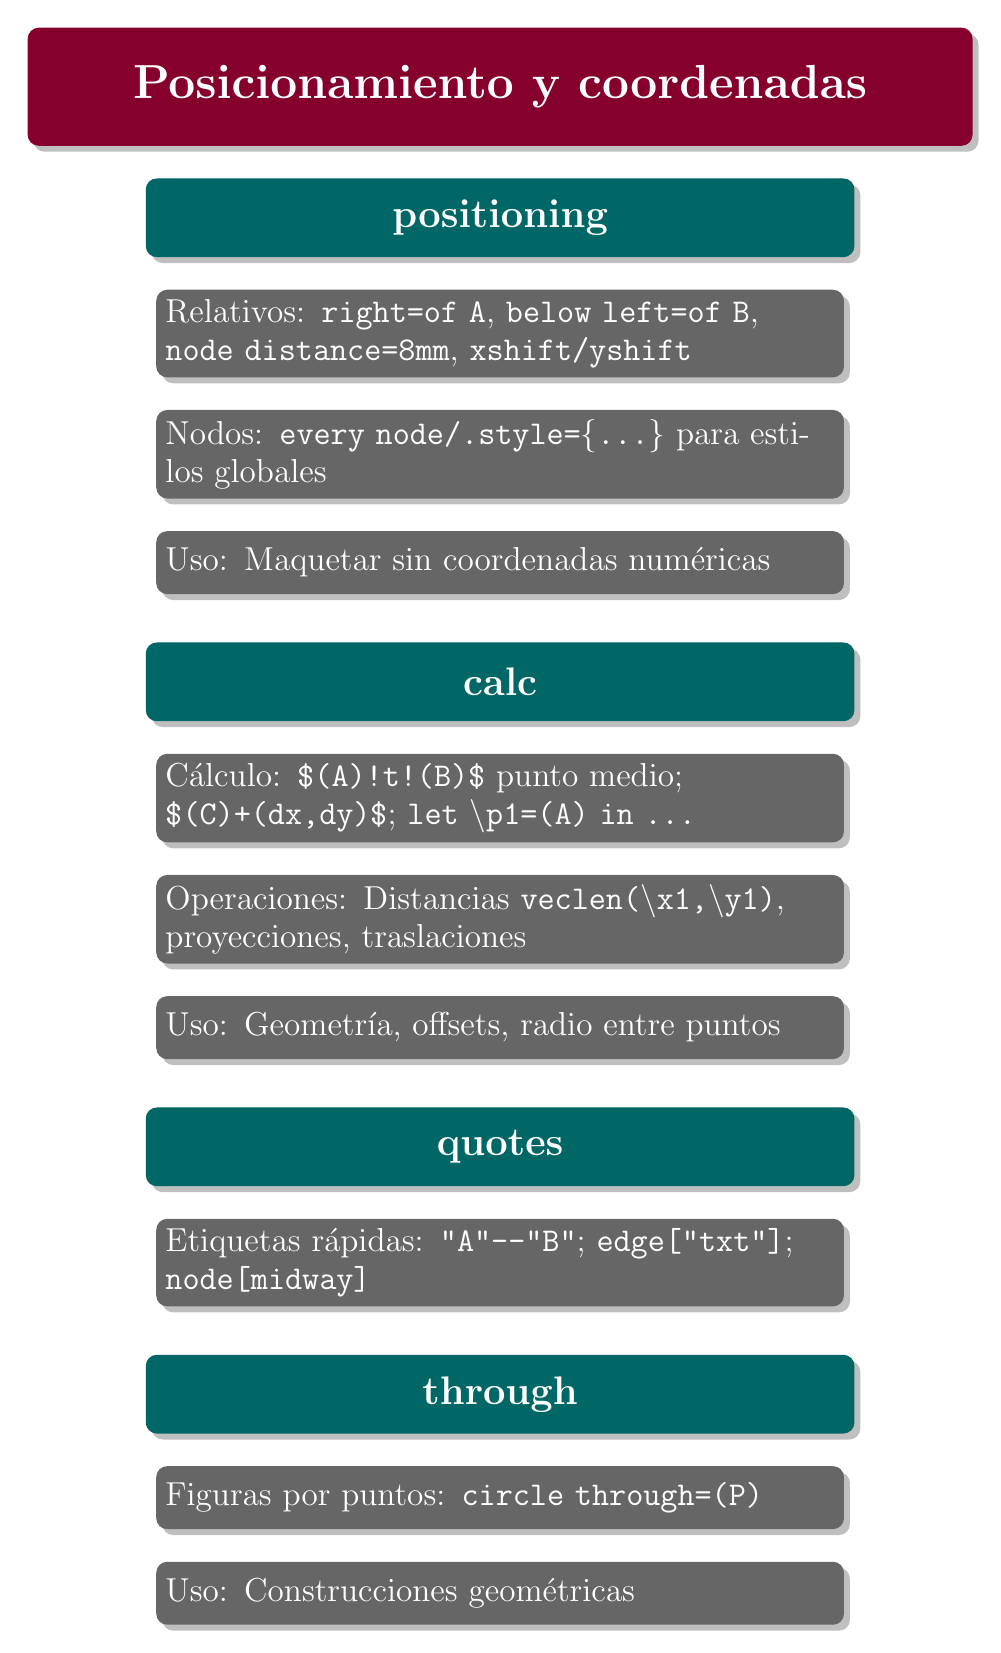
\begin{tikzpicture}[node distance=0.4cm]
			\node[titulo] (root) {Posicionamiento y coordenadas};
			
			\node[nivel1, below=of root] (pos) {positioning};
			\node[nivel2, below=of pos] (p1) {Relativos: \texttt{right=of A}, \texttt{below left=of B}, \texttt{node distance=8mm}, \texttt{xshift/yshift}};
			\node[nivel2, below=of p1] (p2) {Nodos: \texttt{every node/.style=\{...\}} para estilos globales};
			\node[nivel2, below=of p2] (p3) {Uso: Maquetar sin coordenadas numéricas};
			
			\node[nivel1, below=0.6cm of p3] (calc) {calc};
			\node[nivel2, below=of calc] (ca1) {Cálculo: \texttt{\$(A)!t!(B)\$} punto medio; \texttt{\$(C)+(dx,dy)\$}; \texttt{let \textbackslash p1=(A) in ...}};
			\node[nivel2, below=of ca1] (ca2) {Operaciones: Distancias \texttt{veclen(\textbackslash x1,\textbackslash y1)}, proyecciones, traslaciones};
			\node[nivel2, below=of ca2] (ca3) {Uso: Geometría, offsets, radio entre puntos};
			
			\node[nivel1, below=0.6cm of ca3] (quotes) {quotes};
			\node[nivel2, below=of quotes] (q1) {Etiquetas rápidas: \texttt{"A"--"B"}; \texttt{edge["txt"]}; \texttt{node[midway]}};
			
			\node[nivel1, below=0.6cm of q1] (through) {through};
			\node[nivel2, below=of through] (t1) {Figuras por puntos: \texttt{circle through=(P)}};
			\node[nivel2, below=of t1] (t2) {Uso: Construcciones geométricas};
		\end{tikzpicture}
	\end{center}
	
	% =========================================================
	\Lam{Lámina 3 — Formas de nodos}
	\begin{center}
		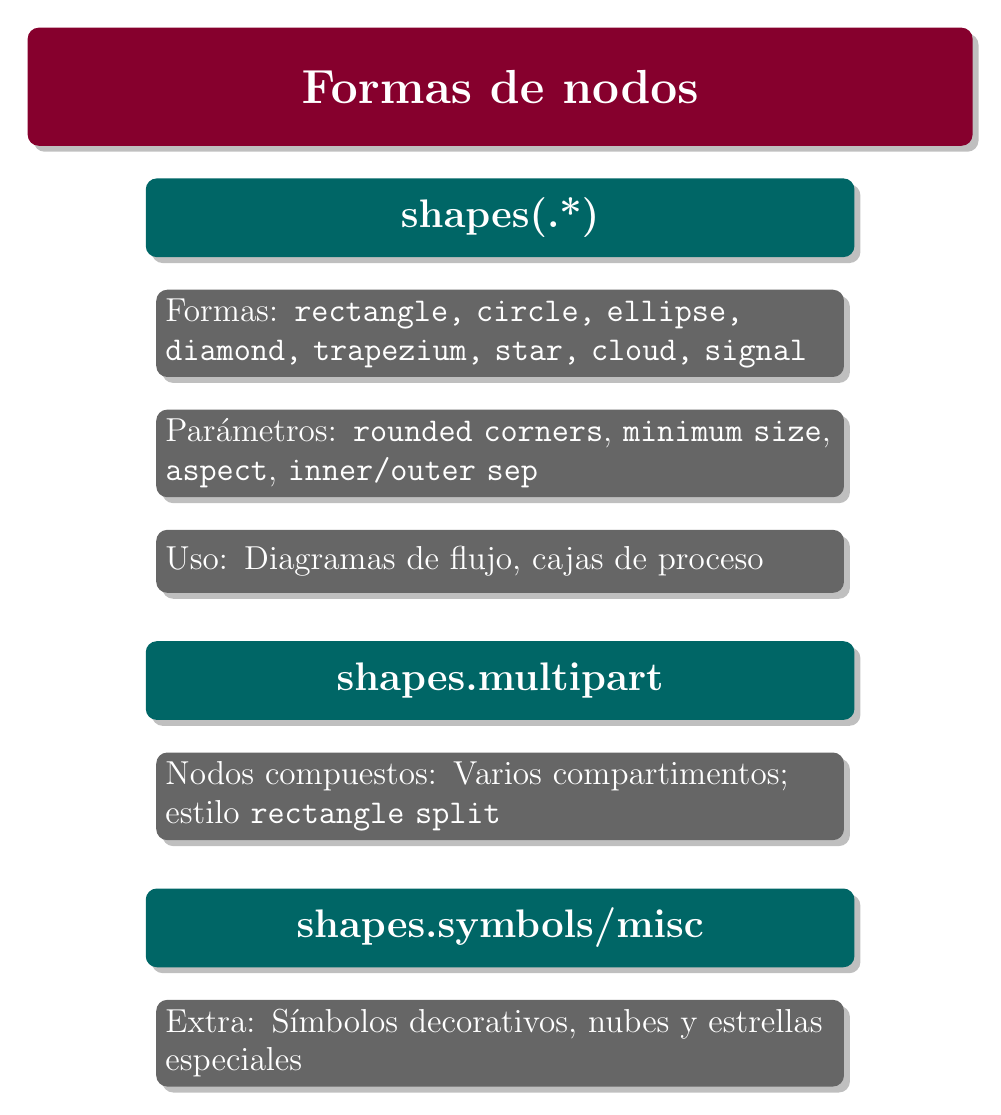
\begin{tikzpicture}[node distance=0.4cm]
			\node[titulo] (root) {Formas de nodos};
			
			\node[nivel1, below=of root] (shapes) {shapes(.*)};
			\node[nivel2, below=of shapes] (s1) {Formas: \texttt{rectangle, circle, ellipse, diamond, trapezium, star, cloud, signal}};
			\node[nivel2, below=of s1] (s2) {Parámetros: \texttt{rounded corners}, \texttt{minimum size}, \texttt{aspect}, \texttt{inner/outer sep}};
			\node[nivel2, below=of s2] (s3) {Uso: Diagramas de flujo, cajas de proceso};
			
			\node[nivel1, below=0.6cm of s3] (multi) {shapes.multipart};
			\node[nivel2, below=of multi] (m1) {Nodos compuestos: Varios compartimentos; estilo \texttt{rectangle split}};
			
			\node[nivel1, below=0.6cm of m1] (symbols) {shapes.symbols/misc};
			\node[nivel2, below=of symbols] (sy1) {Extra: Símbolos decorativos, nubes y estrellas especiales};
		\end{tikzpicture}
	\end{center}
	
	% =========================================================
	\Lam{Lámina 4 — Rellenos y estilos}
	\begin{center}
		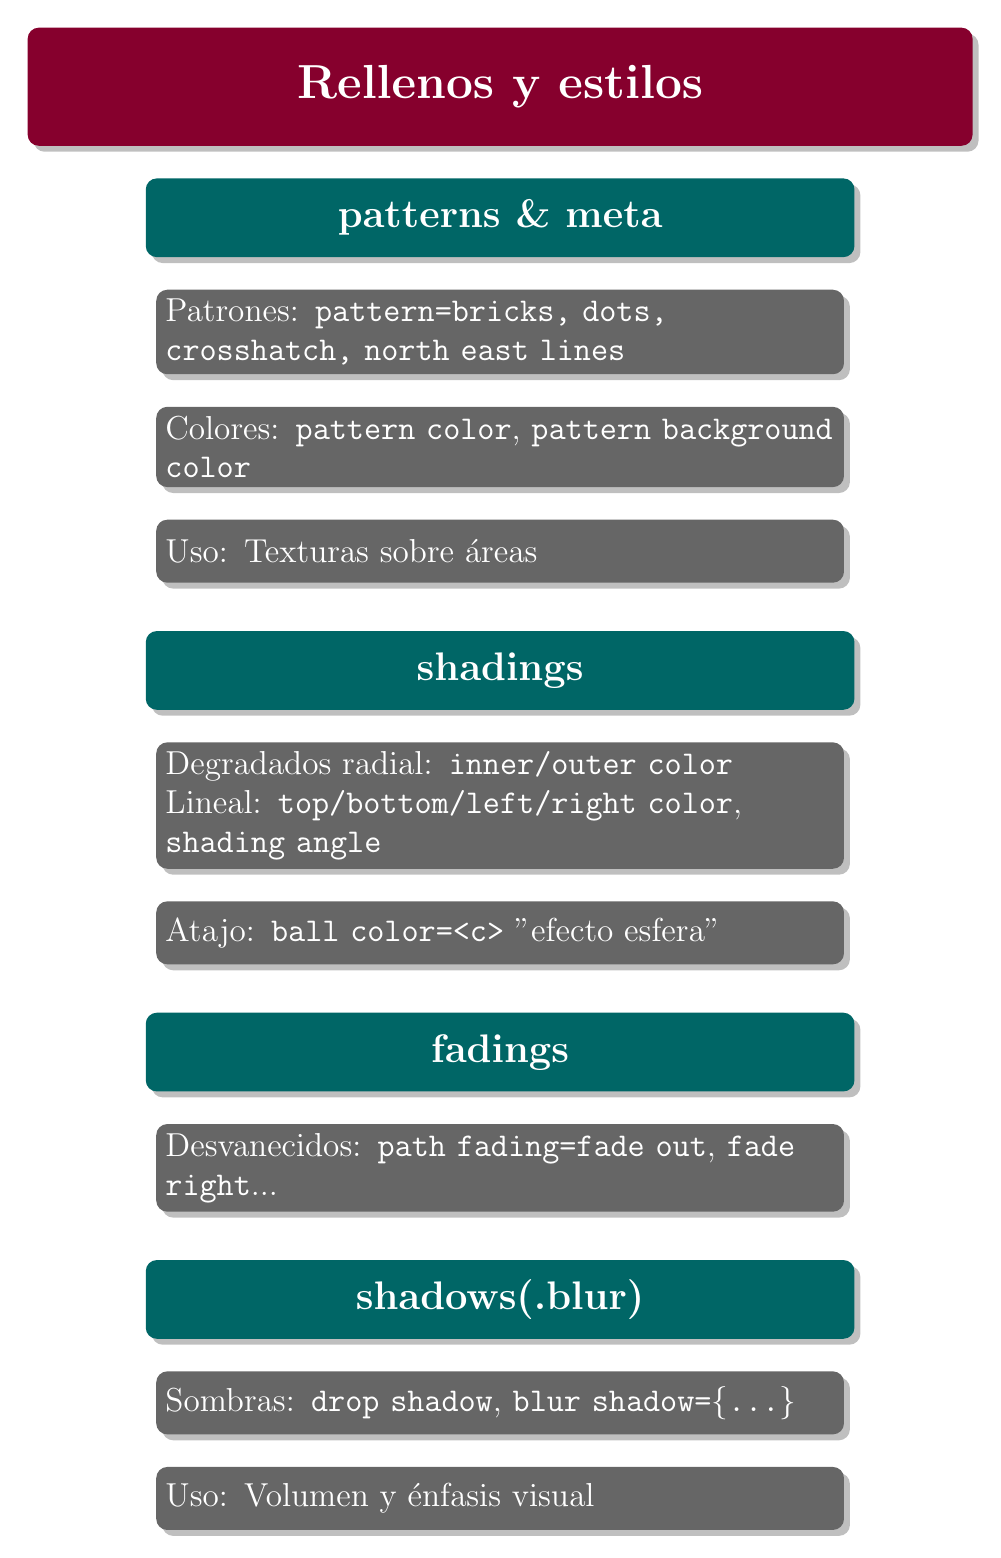
\begin{tikzpicture}[node distance=0.4cm]
			\node[titulo] (root) {Rellenos y estilos};
			
			\node[nivel1, below=of root] (patterns) {patterns \& meta};
			\node[nivel2, below=of patterns] (pa1) {Patrones: \texttt{pattern=bricks, dots, crosshatch, north east lines}};
			\node[nivel2, below=of pa1] (pa2) {Colores: \texttt{pattern color}, \texttt{pattern background color}};
			\node[nivel2, below=of pa2] (pa3) {Uso: Texturas sobre áreas};
			
			\node[nivel1, below=0.6cm of pa3] (shadings) {shadings};
			\node[nivel2, below=of shadings] (sh1) {Degradados radial: \texttt{inner/outer color}\\
				Lineal: \texttt{top/bottom/left/right color}, \texttt{shading angle}};
			\node[nivel2, below=of sh1] (sh2) {Atajo: \texttt{ball color=<c>} "efecto esfera"};
			
			\node[nivel1, below=0.6cm of sh2] (fadings) {fadings};
			\node[nivel2, below=of fadings] (f1) {Desvanecidos: \texttt{path fading=fade out}, \texttt{fade right}...};
			
			\node[nivel1, below=0.6cm of f1] (shadows) {shadows(.blur)};
			\node[nivel2, below=of shadows] (sha1) {Sombras: \texttt{drop shadow}, \texttt{blur shadow=\{...\}}};
			\node[nivel2, below=of sha1] (sha2) {Uso: Volumen y énfasis visual};
		\end{tikzpicture}
	\end{center}
	
	% =========================================================
	\Lam{Lámina 5 — Capas y fondos}
	\begin{center}
		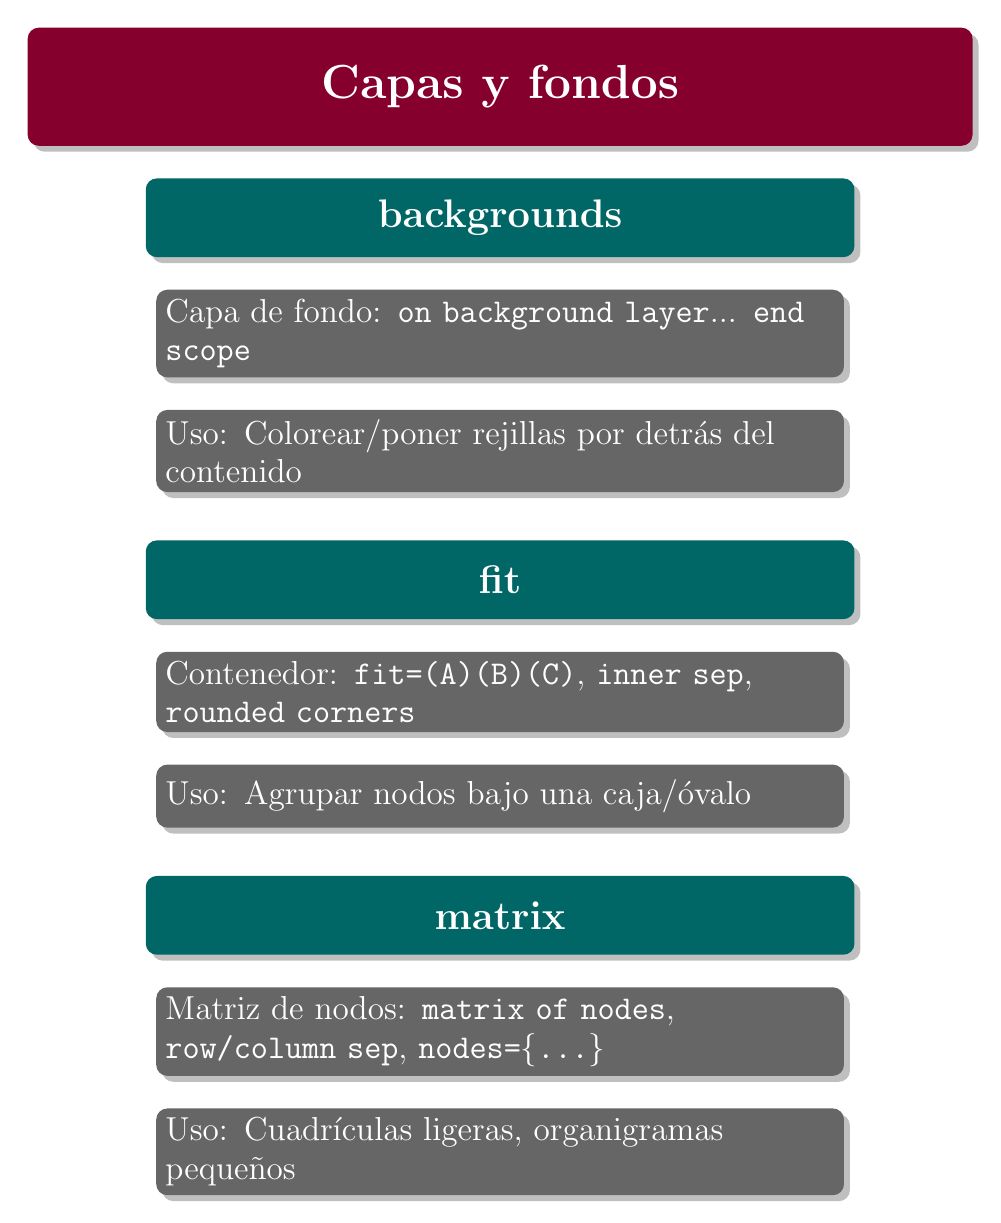
\begin{tikzpicture}[node distance=0.4cm]
			\node[titulo] (root) {Capas y fondos};
			
			\node[nivel1, below=of root] (backgrounds) {backgrounds};
			\node[nivel2, below=of backgrounds] (bg1) {Capa de fondo: \texttt{on background layer}... \texttt{end scope}};
			\node[nivel2, below=of bg1] (bg2) {Uso: Colorear/poner rejillas por detrás del contenido};
			
			\node[nivel1, below=0.6cm of bg2] (fit) {fit};
			\node[nivel2, below=of fit] (fi1) {Contenedor: \texttt{fit=(A)(B)(C)}, \texttt{inner sep}, \texttt{rounded corners}};
			\node[nivel2, below=of fi1] (fi2) {Uso: Agrupar nodos bajo una caja/óvalo};
			
			\node[nivel1, below=0.6cm of fi2] (matrix) {matrix};
			\node[nivel2, below=of matrix] (ma1) {Matriz de nodos: \texttt{matrix of nodes}, \texttt{row/column sep}, \texttt{nodes=\{...\}}};
			\node[nivel2, below=of ma1] (ma2) {Uso: Cuadrículas ligeras, organigramas pequeños};
		\end{tikzpicture}
	\end{center}
	
	% =========================================================
	\Lam{Lámina 6 — Decoraciones}
	\begin{center}
		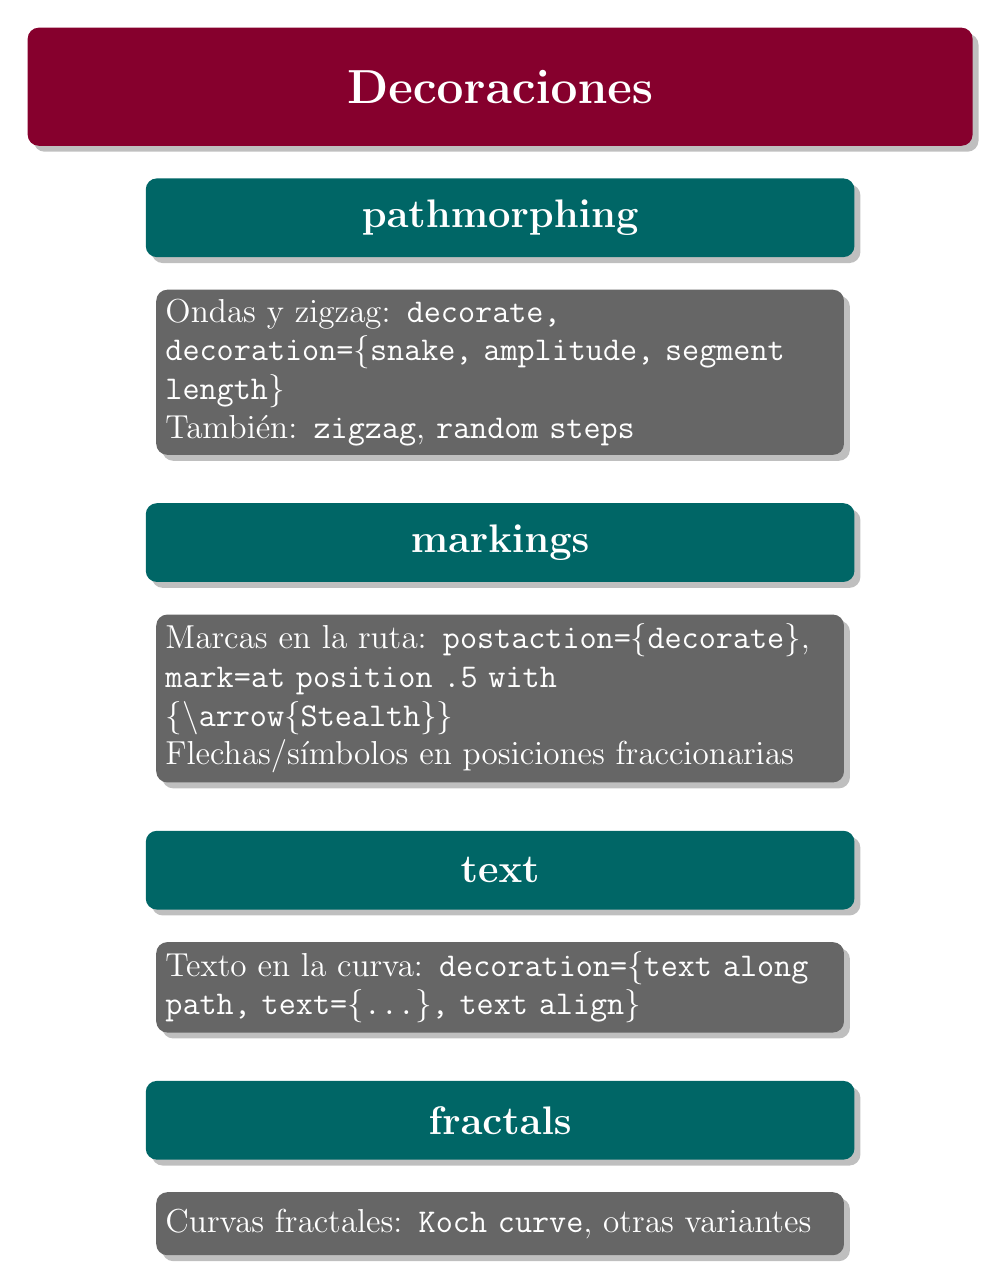
\begin{tikzpicture}[node distance=0.4cm]
			\node[titulo] (root) {Decoraciones};
			
			\node[nivel1, below=of root] (morphing) {pathmorphing};
			\node[nivel2, below=of morphing] (mo1) {Ondas y zigzag: \texttt{decorate, decoration=\{snake, amplitude, segment length\}}\\
				También: \texttt{zigzag}, \texttt{random steps}};
			
			\node[nivel1, below=0.6cm of mo1] (markings) {markings};
			\node[nivel2, below=of markings] (mark1) {Marcas en la ruta: \texttt{postaction=\{decorate\}}, \texttt{mark=at position .5 with \{\textbackslash arrow\{Stealth\}\}}\\
				Flechas/símbolos en posiciones fraccionarias};
			
			\node[nivel1, below=0.6cm of mark1] (text) {text};
			\node[nivel2, below=of text] (te1) {Texto en la curva: \texttt{decoration=\{text along path, text=\{...\}, text align\}}};
			
			\node[nivel1, below=0.6cm of te1] (fractals) {fractals};
			\node[nivel2, below=of fractals] (fr1) {Curvas fractales: \texttt{Koch curve}, otras variantes};
		\end{tikzpicture}
	\end{center}
	
	% =========================================================
	\Lam{Lámina 7 — Grafos y árboles}
	\begin{center}
		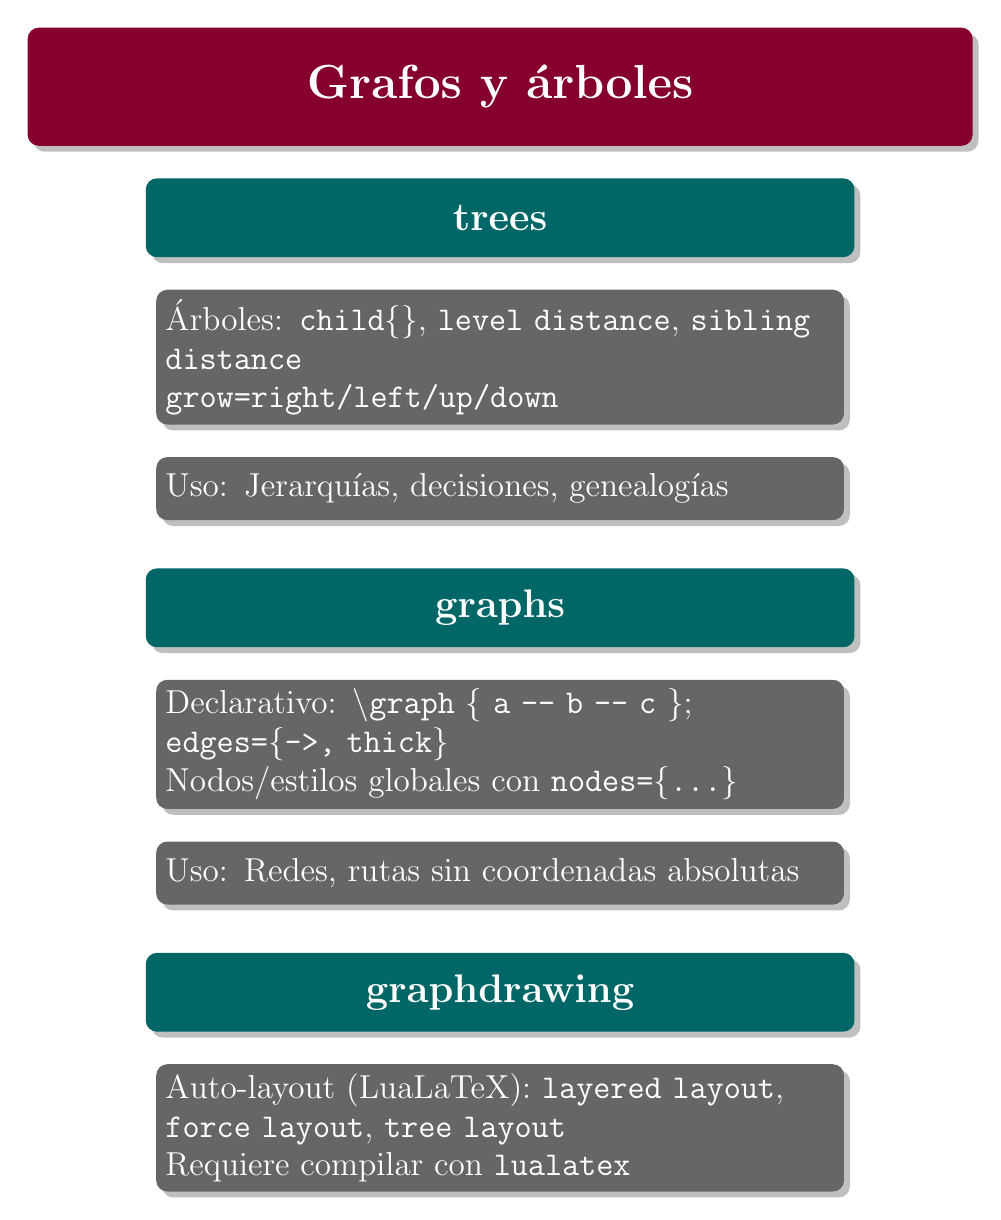
\begin{tikzpicture}[node distance=0.4cm]
			\node[titulo] (root) {Grafos y árboles};
			
			\node[nivel1, below=of root] (trees) {trees};
			\node[nivel2, below=of trees] (tr1) {Árboles: \texttt{child\{\}}, \texttt{level distance}, \texttt{sibling distance}\\
				\texttt{grow=right/left/up/down}};
			\node[nivel2, below=of tr1] (tr2) {Uso: Jerarquías, decisiones, genealogías};
			
			\node[nivel1, below=0.6cm of tr2] (graphs) {graphs};
			\node[nivel2, below=of graphs] (gr1) {Declarativo: \texttt{\textbackslash graph \{ a -- b -- c \}}; \texttt{edges=\{->, thick\}}\\
				Nodos/estilos globales con \texttt{nodes=\{...\}}};
			\node[nivel2, below=of gr1] (gr2) {Uso: Redes, rutas sin coordenadas absolutas};
			
			\node[nivel1, below=0.6cm of gr2] (drawing) {graphdrawing};
			\node[nivel2, below=of drawing] (gd1) {Auto-layout (LuaLaTeX): \texttt{layered layout}, \texttt{force layout}, \texttt{tree layout}\\
				Requiere compilar con \texttt{lualatex}};
		\end{tikzpicture}
	\end{center}
	
\end{document}